%\documentclass[twoside,a4paper,ngerman, german,12pt,authoryear,openright]{book}
\documentclass[twoside,english,12pt,authoryear,openright]{book}
\usepackage{geometry} % see geometry.pdf on how to lay out the page. There's lots.
\geometry{a4paper} % or letter or a5paper or ... etc

\usepackage{graphicx}
\usepackage{pslatex}
\usepackage[utf8]{inputenc} 
\usepackage[T1]{fontenc}
\usepackage[english]{babel}
\usepackage{a4wide}
\usepackage{fancyhdr}


\usepackage{listings}
\usepackage{courier}
\usepackage{color}
\lstset{
         basicstyle=\scriptsize\ttfamily, % Standardschrift
%         numbers=left,               % Ort der Zeilennummern
         numberstyle=\tiny,          % Stil der Zeilennummern
%         stepnumber=2,               % Abstand zwischen den Zeilennummern
         numbersep=5pt,              % Abstand der Nummern zum Text
         tabsize=4,                  % Groesse von Tabs
         extendedchars=true,         %
%         breaklines=true,            % Zeilen werden Umgebrochen
%         keywordstyle=\color{blue}\textbf,
         keywordstyle=\ttfamily,
%         frame=tblr,         
 %        keywordstyle=[1]\textbf,    % Stil der Keywords
 %        keywordstyle=[2]\textbf,    %
 %        keywordstyle=[3]\textbf,    %
 %        keywordstyle=[4]\textbf,   \sqrt{\sqrt{}} %
%         stringstyle=\color{white}\ttfamily, % Farbe der String
         showspaces=false,           % Leerzeichen anzeigen ?
         showtabs=false,             % Tabs anzeigen ?
         xleftmargin=17pt,
         framextopmargin=17pt,
%         framexleftmargin=17pt,
         framexleftmargin=3pt,
         framexrightmargin=5pt,
         framexbottommargin=4pt,
%         backgroundcolor=\color{lightgray},
         showstringspaces=true      % Leerzeichen in Strings anzeigen ?        
 }
 \lstset{language=C++}

\usepackage{hyperref}

\selectlanguage{english}

\pagestyle{fancy}
\setcounter{secnumdepth}{3}
\setcounter{tocdepth}{3}
\setlength\parskip{\medskipamount}
\setlength\parindent{0pt}

\makeatletter
\makeatother

\newcommand{\at}{\textit{ATmega8} }

\begin{document}
\inputencoding{utf8}

\title{Cookbook for Assembly Programming with Arduino and plain 8bit Atmel AVR Micro Controllers}

\author{Felix Morgner and Manfred Morgner}


\maketitle

This book is ongoing work. If you find errors, typos, other mistakes, please get in touch with us. We are always happy to be shown better ways, clearer views, faster solutions, lesser errors ... you name it.

If you wish to follow our ways, it would be a good idea to get a copy of  ,ATMEL 8bit AVR instruction set manual':

\url{http://www.atmel.com/dyn/resources/prod_documents/doc0856.pdf}

In our book we will not explain the commands we are using because all explanation is already worded out in the named document. Clearly we will discuss why we are using specific commands if there are known (as in the context of the book) alternatives.

This book is mainly based on \at because we need to push aside micro controller model specifics. At some point we have to start to deal with this problem but we try to prevent this from happening as hard as we possibly can.

We are more destined to show what can be made and done with a small micro controller. It's clear for us, that more powerful platforms are available for a similar price. But our believe is, that learning Assembler Programming leaves deeper traces if the result of ones work is amazing in face of the used hardware, like a music instrument out of a micro controller some wire and some resistors.

This book is about Assembler Programming. We do not share the view that Assembler Programming will rescue the world. Each programming language has its purpose and some of them are useful too. The reader of this book wishes to learn Assembler Programming by example and has a tendency to experiment with the real thing. We try to satisfy this kind of reader by keeping the circuits simple and so price and requirements low.


\tableofcontents{}
\listoffigures{}
% \listoftables{}

\part{Simple Samples}

\chapter{Light}

In this chapter we will demonstrate the basics of assembly programming with AVR Micro Controllers. These samples will only require the simplest of additional hardware. If you use an Arduino, you will need only a simple wire for the first examples and the very first example nothings more than a powered Arduino.

\begin{figure}[htbp]
  \centering
  \includegraphics[width=120mm]{Media/www-arduino-cc_ArduinoUnoFront.jpeg}
  \caption{Arduino Uno}
  \label{ArduinoUnoFront}
\end{figure}



\begin{figure}[htbp]
  \centering
  \includegraphics[width=120mm]{LED/S000_let-there-be-light_Circuit_schema.png}
  \caption{Light - Schema}
  \label{atmega8-let-there-be-light-schema}
\end{figure}

If not, you may build a circuit like in figure \ref{atmega8-basic-schema} on page \pageref{atmega8-basic-schema}. The breadboard layout is shown in file \texttt{LED/S000\_LED-Basic-Circuit.fz} in Fritzing file format.

As you may find out, we are focused on Free and Open Source Software. All published program code here is Free Software, the book itself and all used attachments are as free as we allowed to make them.

Also we will prevent usage of non free 'things' as hard as we can. We will not force anyone to use non free products to follow our ways. On of our main goals is an intellectual contribution to the world of Free Thinking, Libre Software and cooperative work.


\section{Let there be light}

The first sample in this chapter is the smallest program I can think of which does something.
This program will switch on the LED on your Arduino on pin 13.

Programming in Assembler means you're in control. But as you know, power requires knowledge and responsibility. If you're entering the world of assembly programming, you have absolute power if you wish to or not. Consequently you need both, knowledge to become responsible.

At first you need to know what 'Arduino pin 13' really means! As consequence of the Arduino design it is not pin 13 on your \at. Knowing this is yet the half way thru. Knowing the pin is a step you need to know if are working with a plain chip. What you need to know is the MC internal addressing for Arduino pin 13. To find out, look at \url{http://arduino.cc/hu/Hacking/PinMapping}. After we know everything we have to know to be responsible, we generate our 8byte machine program that will set our 'LED 13' under power.

\begin{lstlisting}
; LED/S000_let-there-be-light.asm

.DEVICE atmega8

.org 0x0000
            rjmp    start 

start:
            sbi     DDRB,         5
            sbi     PORTB,        5
            
main:
            rjmp    main
\end{lstlisting}

As simple as the program is, I believe there is some need for explanation.

At first we have to declare the type of micro controller we are intuited to use with the program. This is necessary because different micro controllers do have different assignments in their inner structure and need different addressing for their components. We do this by:

\begin{lstlisting}
.DEVICE atmega8
\end{lstlisting}

Next we need to declare where our world will start. Funny thing is, we done really know! So we are forced to use symbols to deal with this necessity. As indicated below, different micro controllers will have different inner values. But not only this, to be honest, where our program lives is due to additional effect a most uncertain thing. We come to this later in the book.

As we are forced to use symbols, we have to do so. We will set a symbol to our programs starting point later and this symbol will be named 'start' in out code. Whatever starts our program it must be informed where to goto to do so:

\begin{lstlisting}
.org 0x0000
            rjmp     start 
\end{lstlisting}

With '.org' (don't forget the leading dot!) we build up a sequence of command positioned at the addressed position. This sequence, some times named a table, is a list of action to be taken for different requests. The only request we have is to start our program and fortunately the entry for this request is expected as the first in our table.

For those who really want to know: The addressing in this table is relative to wherever it is placed in real life! So it always starts with 0. Strictly speaking, at this point we already enter the realms of a dreamworld. We don't know what really happens! But sometimes this is irrelevant

To declare our first magic point, we only need to postulate:

\begin{lstlisting}
start:
\end{lstlisting}

'start:'  is a label and represent the final address for the first memory position used afterwards. In our case the address of the first command in our program.

The next label is already behind all things we need to do in our program. It is the starting point of an unconditional infinite loop. This sequence is necessary because the processor (CPU) of our MC is running as long as it has power. We can't stop it, so we have to lead it into a controlled way of doing nothing because we don't wish that our MC does anything after it did all things we expected it to do.

Between 'start:' und 'main:' is our program. I call this the 'first form of a standard program'. A program which runs ones after the system awakes. Such program may be of limited use, but not completely useless. And the schema of this 'first form' is the basic schema of all derived form. The program 

\begin{itemize}
  \item  starts
  \item  does something
  \item  loops forever, possibly doing something
\end{itemize}

If the program does something in the 'infinite loop' then this may be called the 'second form of a standard program'. A third form should be expected to pop into existence later on. But anyway. Our program of the first form is specifically designed to show some important rules for good programming.

The two commands which full fill our programs mission will do two things:

\begin{itemize}
  \item  declare pin 5 at PORTB as output pin
  \item  set pin 5 at PORTB under power to enlighten our LED
\end{itemize}

\begin{lstlisting}
            sbi     DDRB,         5
            sbi     PORTB,        5
\end{lstlisting}

Finally the never ending loop:

\begin{lstlisting}
main:
            rjmp    main
\end{lstlisting}

This is all the program does and there is nothing more about it. You will discover, that this program demonstrates prudence and thrift. But for the moment, our knowledge is insufficient to explain it.



!en \section{Get me on, leave me off}
!de \section{Mach' mich an, lass' mich aus}

!en X

!de Zuerst die erweiterte Schaltung

\begin{figure}[htbp]
  \centering
  \includegraphics[width=120mm]{LED/S002_get-me-on-get-me-off_Circuit_schema.png}
!en   \caption{Get me on, get me off - Schema}
!de   \caption{Mach' mich an, lass' mich aus - Schaltplan}
  \label{atmega8-get-me-on-get-me-off-schema}
  \label{atmega8-get-me-on-get-me-off-schema}
\end{figure}


!en Second the code

!de Anschliessend das Programm


\begin{lstlisting}
; LED/S002_get-me-on-get-me-off.asm

.DEVICE atmega8

.org 0x0000
            rjmp     start

start:
            sbi     DDRB,         5
            cbi     DDRB,         0
            sbi     PORTB,        0

main:
            sbic    PINB,         0 ; 1 cycles if false or 2
            rjmp    led_on          ; 2 cycles
            cbi     PORTB,        5 ; 1 cycle
            rjmp    led_ok          ; 2 cycles
led_on:
            sbi     PORTB,        5 ; 1 cycle
led_ok:
            rjmp    main            ; 2 cycles
\end{lstlisting}

!en X

!de Wie zu vermuten war, handelt es sich hier bereits ein Programm der 'Zweiten Form'. Es tut nicht nur etwas \textit{vor} der Endlosschleife, sondern ebenfalls etwas darin. Dieses Programm hat wirklich viel zu tun, wie noch sehen werden.



!en X

!de Der erste Unterschied zum vorherigen Programm ist, dass wir ein zusätzliches Bein benutzen, diesmal um ein Eingangssignal zu erkennen. Um dieses Bein, Bit 0 an Port B = Bein 14 am MC, auf den Input Modus zu schalten, senden wir eine \texttt{0} an das entsprechende 'Data Direction Register' (\texttt{DDR}), also \texttt{cbi DDRB, 0}. Ausserdem senden wir eine \texttt{1} auf das Bit am entsprechenden Port, \texttt{sbi PORTB, 1}. Was im Ausgabemodus bedeuten würde 'Schalte VCC an das Bein', heisst im Eingabemodus: 'Schalte den pull-up-Widerstand\footnote{Ein pull-up-Widerstand ist ein Widerstand, der dazu benutzt wird, um den Signalpegel an einem Bein 'hoch' (auf VCC) zu legen = \texttt{1}. Er dient dazu um an einem Eingangsbein auch dann einen stabilen Zustand zu erreichen, wenn kein Element angeschlossen ist.} zu'.



!en X

!de Danach können wir vom Eingangsbein den Status 'EIN' oder '1' lesen. Um eine Reaktion am MC zu erreichen und das Eingangssignal auf 'AUS' oder '0' zu setzen, müssen wir das Beim auf GND ziehen.



!en X

!de Wenn wir das machen, schaltet unser Programm das Licht aus solange wir das Eingangsbein auf Masse legen. Das ist nicht direkt eine Anwendung mit der wir gross angeben können. Für uns ist es dennoch grossartig weil wir verstehen was passiert!



!en If you follow the programs flow:

%de Das Programm läuft folgendermassen ab:

\begin{enumerate}
!en   \item Initialise system and all connected devices
!de   \item Initialisiere das System und die angeschlossenen Geräte
!en   \item (*) Read bit 0
!de   \item (*) Lese Bit 0
!en   \item Set bit 5 accordingly
!de   \item Setze Bit 5 entsprechend
!en   \item Continue with (*)
!de   \item Weiter bei (*)
\end{enumerate}



!en X

!de Jemand, der dieses Programm unter dem Blickwinkel der Sparsamkeit betrachtet, wird sich womöglich fragen, wieso ständig das gleiche Signal auf das Ausgabebit ausgegeben wird. Wenn wir einmal grob annehmen, dass unser Programm das Eingangsbit ca. eine Million mal pro Sekunde liest (eher 8 Mio. mal bei 8MHz ), ist einzusehen, dass ein Mensch mit einem Tasten kaum 'Last' für unseren MC erzeugen kann. Wenn ein Mensch auf den Schalter einhämmert so schnell er kann, passiert aus der Sicht des Micro Controllers so gut wir gar nichts, das Signal ändert sich auf diese Weise für den MC in historischen Zeiträumen.


!en X

!de Die tatsächliche Abfragefrequenz ist möglicher Weise unterschiedlich für die beiden Systemzuständen (Signal \texttt{1} oder \texttt{0}). Wir rechnen kurz nach:

\begin{enumerate}
!en   \item X
!de   \item Signal = '\texttt{1}' entspricht 5 Zyklen
!en   \item X
!de   \item Signal = '\texttt{0}' entspricht 7 Zyklen
\end{enumerate}



!en X

!de Die Schleifendurchlauffrequenz können wir einfach berechnen, indem wir die Taktfrequenz des Prozessors durch die Anzahl der erforderlichen Taktzyklen für einen Schleifendurchlauf teilen.

\begin{equation}
f_{Loop} = \frac{f_{CPU}}{d}
\end{equation}

!en X

!de Wobei d die 'Dauer' eines Schleifendurchlaufs in Zyklen pro Schleifendurchlauf ist. Das bedeutet, dass der MC ohne Druck auf den Taster 8/5 Mio. Mal pro Sekunde den Schaltzustand des Tasters anfragt und bei gedrücktem Taster 8/7 Mio. Mal pro Sekunde.


!en X

!de Solche Abfragefrequenzen sind im Allgemeinen unsinnig. Es gibt Fälle, in denen auch die Bedienung von Tasten durch Menschen zeitkritisch sind, wenn es sich um Musikinstrumente handelt, kommt es auf Millisekunden an. Aber um ein Licht einzuschalten, genügen problemlos 30 Schleifendurchläufe je Sekunde. Mehr kann der Mensch ohnehin nicht erkennen. Kann man das System also optimieren? Wir glauben nicht.



!en X

!de Gibt es andere Lösungen? Ja, die gibt es!



!en \subsection{CPU Frequency}
!de \subsection{CPU Frequenz anpassen}

!en X

!de Wir könnten die Taktfrequenz, mit der die CPU operiert senken. Je nach Einsatzfall kann das tatsächlich helfen, Energie zu sparen, wäre aber damit verbunden, die Rechenleistung des Systems zu reduzieren und kann nachteilig wirken, wenn zusätzliche Aufgaben erledigt werden.



!en X

!de Es kann allerdings nicht schaden, sich in jedem Fall Gedanken über die Taktfrequenzen zu machen, die in einem Micro Controller zusammenkommen. Sowohl nach unten wie auch nach oben. Letztlich beeinflusst eine solche Entscheidung auch die Auswahl des Micro Controllers als solchem.



\subsection{Interrupts}

!en X

!de Vielleicht könnte man auch Interrupts verwenden, um die Signalisierung des Schalterstatus umzukehren. Der Mikroprozessor erledigt dann die Abfrage für uns und signalisiert dem Programm aktiv, dass der Knopf gedrückt wurde. Dieses Verfahren macht einen ruhigeren Eindruck, läuft technisch aber auf das gleiche Prinzip hinaus, mit dem Unterschied, dass wir einen grossen Aufwand zur Initialisierung der Interruptauslösung betreiben müssten, ohne dass die CPU weniger rotieren hätte. Die Hauptprogrammschleife wäre dann leer. Doch sie würde sich auch leer mir dem vollen CPU Takt um sich selbst drehen.



!en X

!de Das heisst, das Programm wird komplizierter - wie wir sehen werden schränkt ein solches Verfahren sogar die Anzahl der Pins ein, die als Schaltereingang benutzt werden können - aber die CPU Last bleibt gleich.


!en X

!de Wirklich nützlich wird dieses Verfahren erst, wenn die CPU abgeschaltet werden könnte, während sie auf einen Interrupt wartet oder - dann sowieso - wenn das Programm parallel noch eine Reihe anderer Aufgaben zu lösen hätte. Beides werden wir noch demonstrieren. Beides ist in der aktuellen Phase aber noch zu komplex.



!en \subsection{X}
!de \subsection{Statusverwaltung}



!en X

!de Wir könnten den zuletzt ausgegebenen Status speichern. Dann könnten wir in der nächsten Programmschleife prüfen ob sich der eingelesene Status zum vorherigen Status geändert hat und nur dann ein Signal an das Bein ausgeben, wenn eine solche Änderung vorliegt. Das könnte uns ersparen, 8/5 oder 8/7 Mio. Mal pro Sekunde den unveränderten Status an die LED auszugeben.



!en X

!de Das klingt gut und einfach, ist es aber leider nicht! Es ist nicht nur nicht einfach, es ist gefährlich, kostspielig und kompliziert. Und es ist effektiv sinnlos weil wir eine Menge Aufwand treiben würden, ohne dass sich wirklich etwas verbessert.



!en X

!de Dieses Konzept ist gefährlich weil das Programm aus dem Rhythmus kommen könnte. Danach würde es falsch herum arbeiten oder überhaupt nicht mehr auf Eingangssignale reagieren.



!en X

!de Es ist kostspielig weil das Programm nicht nur viel grösser würde, wir würden ausserdem ein CPU Register verbrauchen (um den Status zu speichern) und wir haben um \at{} total nur 32 Stück von denen nur die Hälfte einfach zu benutzen ist!



!en X

!de Und es ist kompliziert weil wir zwei unabhängige Einheiten im Gleichlauf halten müssen (das Licht und das Statusregister) um vielleicht einen Effekt zu erzielen. Das ist ein grosses Risiko und ein Nachteil gegenüber der vorliegenden Lösung.



!en X

!de Aus diesen Gründen liegen wir vielleicht nicht falsch mit der Vermutung, dass die Entwickler unseres Micro Controllers ihren Chip so entwickelt haben, dass in Wirklichkeit gar nichts gemacht wird, wenn wir eine '1' auf ein Steuerbit senden, dass bereit auf '1' gesetzt ist. Diese Form der Optimierung darf man erwarten.



!en X

!de In der Summe heisst das, dass wir momentan am Ende unsere Möglichkeiten sind Wir müssen hier also bei der vorliegenden Lösung bleiben. Die Vorgeschlagenen Ansätze werden später allerdings noch aktuell werden.
\section{Stable Decisions}

For the next step we need to do something more useful. But we stay with the 'second form of a standard program': A program that does something in its infinite loop.

This program stores one of two states ;-) and sets the light on or off, keeping it according to the stored status. This explanation is slightly wrong. I try it again.

This program recognises an input signal consisting of two phases. A complete input signal consist of a LOW phase starting from a HIGH phase followed by the next HIGH phase. The signal ends with entering the HIGH phase again. We are interested only in change, as we always should.

If the Input signal changes from HIGH to LOW, our program changes the light from its current status to the opposite status. If the light was ON it will be set to OFF and vice versa. The status is only changed as reaction of changing the Input from HIGH to LOW because 'no action' at the Input device leads to HIGH status in the input bit as result of using an internal pull-up resistor who does what he is called - he pulls the input signal up to HIGH.

The electrical signal we are waiting for with our micro controller on our input bit is: Pulling the status down to LOW (GND). We may phrase:

\begin{center}
The \emph{Signal} we are waiting for is the \emph{Change} form HIGH to LOW.
\end{center}


So for the first time we have to be aware of a dynamic process. If the change of the status is the signal, then we have to recognise if the status is change. If a status appears after the opposite status was recognised - in the past - which is then no more present (!) we have to deal with 'historical' status management and so for the first time we remember a status from one processing cycle to the next.

Finally this here is the Code to do it:

\begin{lstlisting}
; LED/S004_stable-decisions.asm

.DEVICE atmega8

.org 0x0000
            rjmp    start

start:
            sbi     DDRB,         5
            cbi     DDRB,         0
            sbi     PORTB,        0

            ldi     r16,          1

main:
            sbic    PINB,         0
            rjmp    led_keep
            tst     r16
            breq    led_ok
            clr     r16
            sbis    PINB,         5
            rjmp    led_on
            cbi     PORTB,        5
            rjmp    led_ok
led_on:
            sbi     PORTB,        5
            rjmp    led_ok
led_keep:
            ldi     r16,          1
led_ok:
            rjmp    main
\end{lstlisting}


As you can see, this Code is not easy to understand. To do better, we add symbolic names to the soup. The basics are easy:

\begin{itemize}
  \item \texttt{.equ} means: 'a name for a value'
  \item \texttt{.def} means: 'a name for an entity'
\end{itemize}

So for example \texttt{DDRB} already is a number. This number is defined in an include file chosen by you device selection. In our case, whatever number is hidden behind the name DDRB it will be our Input/Output control port. So the name will be \texttt{ctl} as prefix for 'control' and \texttt{IO} short for Input\&Output.

In another sample \texttt{bit} stands for 'bit number' and \texttt{Input} for 'Input' which makes \texttt{bitInput}, the bit where we read the input status.

You may define you own naming convention which better should hold throughout your project.

\begin{lstlisting}
; LED/S005_stable-decisions+symbols.asm

.DEVICE atmega8

.equ ctlIO     = DDRB    ; DDRB  is our I/O control register
.equ prtIO     = PORTB   ; PORTB is our I/O output port register
.equ pinIO     = PINB    ; PINB  is our I/O input pin register

.equ bitOutput = 5       ; bit 5 is our output bit
.equ bitInput  = 0       ; bit 0 is our input bit

.equ FALSE     = 0       ; 0 will be FALSE or OFF
.equ TRUE      = 1       ; 1 will be TRUE  or ON

.def bStatus   = r16     ; the last state will be stored in 'r16'
\end{lstlisting}

As you may not have expected, this makes the soup - or code - somehow better readable and much easier to understand. Now it looks more like a higher language:

\begin{lstlisting}
.org 0x0000
            rjmp    start

start:
            sbi     ctlIO,        bitOutput
            cbi     ctlIO,        bitInput
            sbi     prtIO,        bitInput

            ldi     bStatus,      HIGH

main:
            sbic    pinIO,        bitInput
            rjmp    led_keep
            tst     bStatus
            breq    led_ok
            clr     bStatus
            sbis    pinIO,        bitOutput
            rjmp    led_on
            cbi     prtIO,        bitOutput
            rjmp    led_ok
led_on:
            sbi     prtIO,        bitOutput
            rjmp    led_ok
led_keep:
            ldi     bStatus,      HIGH
led_ok:
            rjmp    main
\end{lstlisting}

Also it provides us with the possibility of changing things with reduced risk. Shortly we had to change the schema a bit to support additional ideas and we changed \texttt{bitInput} from 4 to 0. Using symbolic names this was much easier and much less risky to do because we only needed to change the definition for \texttt{bitInput}!

Even if symbols make a better reading than constants, it seems not really to be easy to follow the program flow. So at first, we should introduce a program flow chart. And for good measure two of them. We need two of them to demonstrate a major point in assembler programming.

We have to take watch about WHAT we wish to do, but equally to about HOW we are going to do it.

\subsection{WHAT to do}

\begin{enumerate}
  \item Initialise system and devices
  \item Wait for the change "input bit was HIGH and became LOW"
  \item Invert LED status
  \item Restart at (2)
\end{enumerate}


\subsection{HOW to do it}

To get an impression on how to it, at first, we take a look at a flow diagram. This diagram shows the program flow.

\begin{figure}[htbp]
  \centering
  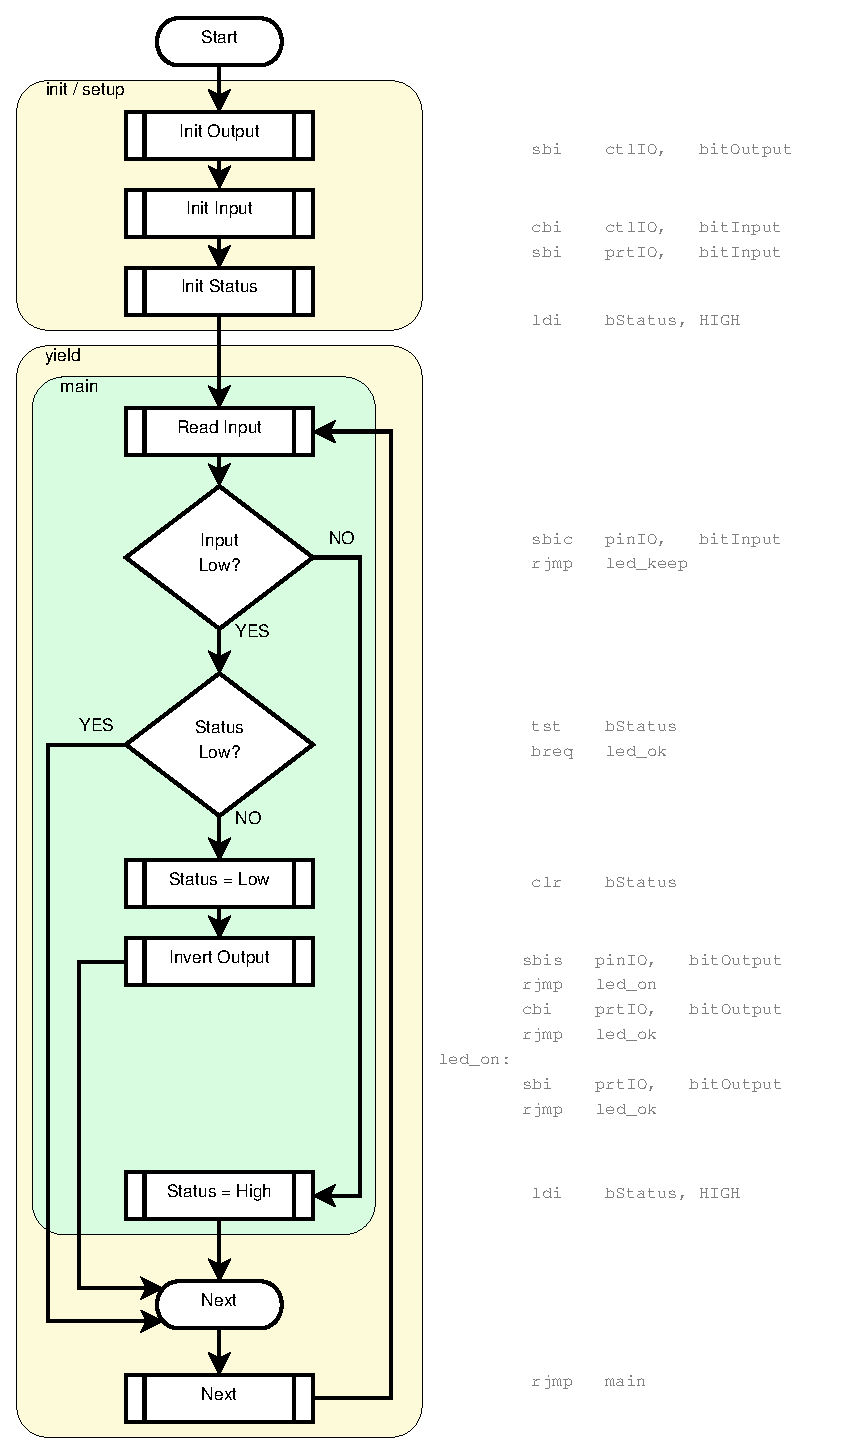
\includegraphics[height=210mm]{LED/S005_stable-decisions+symbols.eps}
  \caption{Stable Decisions - Flow Diagram}
  \label{S005FlowDiagam}
\end{figure}

As you may have found out until now, dealing with the 'human device interface' is the most complicated thing in informatics. It starts with the unbearable slowness of bio entities and does not end with humans expectations against machines. Which means the user is problem number one in software development and for this has to be the main focus! Otherwise your product will not be accepted by those who should pay our wages!

\subsubsection{Slow users}

A living entity presses a button and our device has to react. Our device may ask the input pin about 1.000.000 times per second. A human for example may do a very short pressing of a button in about 0.2 seconds. Which means, our System reads the status 'button pressed' about 200.000 times during our humans action. But what the human expects is:

\begin{center}
Change the light ones as I press (in my view) the button ones!
\end{center}

A problem we will not deal with in this phase of our development is, that electric switches may flicker during status change. Flickery leads to problems because it will generate random additional signals during the action phase. In general this is dealt with by electronically measures. Therefore we simply have to ensure that changing the LEDs status only happens ones per button press action and we will ignore any flickery event by not doing anything about it.

\subsubsection{Fast feedback}

Our feedback device is the light we control. We have no display oder acoustic device to us as feedback but the very same object that goes to be controlled. User feedback therefore simply means to manipulate the status of the light. Even if its cool in movies to do anything without any visible feedback, real living bio entities require 'immediate feedback' for every action. Otherwise they run into problems.


\begin{figure}[htbp]
  \centering
  \includegraphics[width=120mm]{LED/S005_stable-decisions_ideal_signal.png}
  \caption{Stable Decisions - Signal Diagram}
  \label{S005SignalDiagam}
\end{figure}

Figure \ref{S005SignalDiagam} shows the signal we have to expect (idealised). You have to remember, that our micro controller reads the 'LOW' status of the signal 100.000 times or more often. We do not measure time! The natural timing unit in micro controllers is cycles. Read cycles, CPU cycles, sensor cycles. This is important to recognise especially because different clock frequencies and different voltage leads to different physical cycle durations. A program that measures a certain event by 1000 cycles will receive 2000 if the clock is doubled up.

Different clock frequencies lead to different CPU dependent cycles. Different voltage may lead to different sensor cycles, depending on the specification of the sensor in question and the characteristics of the signal to measure. Further, different voltage may lead to different absolute sensor signals, but this is another chapter.

The signal we need to recognise at the moment is the switch from HIGH to LOW and back again. The LOW level will stay for an undefined time / amount of measure cycles. What we have to focus on is the change of the signal!

To deal with this there are only two moments in all this 'endless' button down phase - between 't1' and 't2' - where it is applicable to really change the LEDs status. At the beginning, as the signal changes from HIGH to LOW (t1) or at the end, where the signal changes from LOW to HIGH again (t2).

To give the human who uses our device (the user) immediate feedback about success or failure of his action, we decide to use the first phase (t1) to do all the action. So we have a simple mission: If the signal is LOW now and was HIGH the last time we looked, we change the LEDs state. This satisfies also the endless LOW state of the input signal and the change from LOW to HIGH where we have to do nothing. Not even accidentally! This way, the human feels his request immediately answered, even if he is unable to comprehend on which grade immediately it real is answered.


\subsection{Finding the event}

To find the event the signal has gone to ground, we have to be aware of the status of the signal from the previous query cycle. Which is easy but expensive. We simply use a register to store the previous input status.

We simply have to check if the last seen status was HIGH as log as the current status is LOW. The status accumulator register follows the status of the input signal after being used to query the change event.

If the one moment we are waiting for passes, we invert the LED status. That's all


\subsection{And some modesty}

In respect of things to come, we have to be modest in our style. The 'endless loop' which keeps the micro controller running and waiting without going wild, will be used for some important things:

\begin{itemize}
  \item It mostly contains the main program
  \item It possibly consist of multiple parts
  \item It consist of an undefined amount of functional separate program parts
\end{itemize}

So we have to ensure, to don't make any shortcut back to the 'main' label. As there can only be one Highlander, there can only be one jump back to 'main'. This jump resides at the very end of the main sequence. Like this:

\begin{lstlisting}
main:

  A_begin:
            block     A or goto to end of block A
  A_end:

  B_begin:
            block     B or goto to end of block B
  B_end:

  C_begin:
            block     C or goto to end of block C
  C_end

mein_end:
            finalise
            rjmp      main
\end{lstlisting}

In our flow diagram one part has to reach the next part regardless of how the program is flowing. The rounded rectangle 'next' represents the central point behind our (currently) one part. This is the position where the next program part would follow in the same manner.


\section{Stable Decisions Triggered}

If you feel a bit uncertain about our solution or if you have the feeling that all this should be made better you may be right. We would not ensure you that the following solution is better under every circumstance, but for some application, there is a much better way.

This was we need to introduce the concept of interrupts.

The magic behind interrupts in micro controllers is much more as in simple CPUs!

Interrupts are special mechanics in processing units to enable the execution of code at a certain time or after a certain event by interrupting the normal processing, doing something else and after this continue whatever was interrupted.

In micro processors this mechanic is much more sophisticated. In micro controllers you may interrupt the system from nothing! Meaning, its possible to nearly shut off the whole system, interrupt it from his deep sleep, let it do something and send it back to sleep.

Such applications are useful if energy resources are small. For example, if you wish to drive your weather station one year on a single AAA cell or less, possibly supported by solar power.

In such applications you wish to reduce power consumption of your system as far as possible. There is no need to let your micro controller do eight million cycles per second if you take a measurement every ten minutes! It may be much better so stop the whole system until the next measurement is to start.

You already my expect it. Such code does not need to loop with full processing power to do nothing, such code really does nothing while waiting:


\section{Light Shift}

Next we will start with showing off. A little bitt at least. We will put three lights in a row and lighten one of them up each time we press the button.

It would be much easier to do this with 8 lights, but here we are. We will keep the existing circuit as untouched as possible and, not at last, we are constantly on he search for a challenge.

So here is the code:

\begin{lstlisting}
; LED/S010_light-shift.asm

.DEVICE atmega8


.equ ctlIO         = DDRB
.equ prtIO         = PORTB
.equ pinIO         = PINB

.equ bitSignal     = 5
.equ bitInput      = 4
.equ bitLightStart = 3

.equ mskLightShift = 0x0E

.equ LOW           = 0
.equ HIGH          = 1

.def bStatus       = r16
.def bTemp         = r17
.def bData         = r18


.org 0x0000
            rjmp    start


start:
            ldi     bTemp,        mskLightShift | 1 << bitSignal
            out     ctlIO,        bTemp
            ldi     bTemp,        1 << bitInput | 1 << bitSignal
            out     prtIO,        bTemp

            ldi     bStatus,      HIGH

main:
            sbic    pinIO,        bitInput
            rjmp    led_keep
            tst     bStatus
            breq    led_ok
            clr     bStatus

            in      bData,        pinIO
            mov     bTemp,        bData
            andi    bData,        0xFF - mskLightShift

            andi    bTemp,        mskLightShift
            lsr     bTemp
            andi    bTemp,        mskLightShift
            brne    shift_ok
            ldi     bTemp,        1 << bitLightStart
shift_ok:
            or      bData,        bTemp
            ori     bData,        1 << bitInput
            out     prtIO,        bData

            rjmp    led_ok
led_keep:
            ldi     bStatus,      HIGH
led_ok:
            rjmp    main
\end{lstlisting}



\chapter{Time}

\section{Instable Elements}

The longest time we tried to avoid the simplest demo in most Arduino beginners sets. The blinking light demo! Some of our readers may have ask themselves where the problem should be. Now is the moment to explain.

We do not want to make a fuss with code we would have to be ashamed of but couldn't bring us to start with timers and interrupts before introducing the most basic principles of programming. Please remember, using assembler language brings us in a position of power which forces us into reliability.

There is no way a reliable programmer would use 4.000.000 NOPs ('no operation' operations) twice to let a light blink ones per second. Also, we hope, no one reading until this point would keep it as responsible to enter a loop, busying our poor micro controller to wait half a second by wasting four million CPU cycles.

So we had to experiment enough to enter the reign of timers and interrupts. Staying our ground not demonstrating bad code, keeping the book pure, we don't show only a part of a single bad example in code. You may remember it in your dreams!

To cut a long story short. Here its the code:

\begin{lstlisting}
; LED/S020_instable-elements.asm

.DEVICE atmega8

.org 0x0000
            rjmp    start 

start:
            sbi     DDRB,         5
            sbi     PORTB,        5
            
main:
            rjmp    main
\end{lstlisting}



\part{External devices}

\chapter{Shift Registers}

\input{Shift-Register/S000_shift-sram}

\end{document}
